\documentclass[acmtog]{acmart}
\usepackage{graphicx}
\usepackage{subfigure}
\usepackage{natbib}
\usepackage{listings}
\usepackage{bm}
\usepackage{amsmath}

\definecolor{blve}{rgb}{0.3372549 , 0.61176471, 0.83921569}
\definecolor{gr33n}{rgb}{0.29019608, 0.7372549, 0.64705882}
\makeatletter
\lst@InstallKeywords k{class}{classstyle}\slshape{classstyle}{}ld
\definecolor{mygray}{rgb}{0.5,0.5,0.5}
\makeatother
\setlength{\headheight}{23.89902pt}
\lstset{
    backgroundcolor=\color{lightgray},       
	breakatwhitespace = false,        
	breaklines = true,                 
	captionpos = b,                    
	commentstyle = \color{mygreen}\bfseries,
	extendedchars = false,             
	frame =shadowbox, 
	framerule=0.5pt,
	keepspaces=true,
	keywordstyle=\color{blue}\bfseries, 
	language = C++,                     
	otherkeywords={string}, 
	numbers=left, 
	numbersep=5pt,
	numberstyle=\tiny\color{mygray},
	rulecolor=\color{black},         
	showspaces=false,  
	showstringspaces=false, 
	showtabs=false,    
	stepnumber=1,         
	stringstyle=\color{mymauve},        
	tabsize=2,          
	title=\lstname                      
}

% Title portion
\title{Assignment 4: {Global Illumination}} 

\author{Name:\quad WeiLiang Sun  \\ student number:\ 2020533010
\\email:\quad sunwl1@shanghaitech.edu.cn}

% Document starts
\begin{document}
\maketitle

\vspace*{2 ex}

\section{Introduction}

This is the assignment 4 of the computer graphics, finishing the following part:\\
\textbf{Part 1. Path tracing with Monte Carlo integration} \\
\textbf{Part 2. Ideal diffuse BRDF and area light source} \\
\textbf{Part 3. Acceleration structure: BVH} \\
\textbf{Bonus Part 1. The ideal specular or glossy specular BRDF} \\
\textbf{Bonus Part 2. The translucent BRDF with refraction} \\
\textbf{Bonus Part 3: SAH tree}

\section{Implementation Details}

\subsection{Path tracing with Monte Carlo integration}

In this part, we are supposed to complete the render and radiance methods. To compute the radiance of each pixel in the image plane, we need to construct paths starting from the camera and compute the Monte Carlo integration along these paths in order to solve the light transportation equation.

\textbf{First part. render function}

In render, what we do first is to generate a ray from the camera to a pixel on the image plane.We are given a beta initialized 1 and a L initialized 0. Then we need to traverse the depth, if the ray hit at a 
position we need to do the radiance function. After all is add up, we divide by spp to get an average result. Finally set this pixel.

\textbf{Second part. radiance function}

This is the most important function in part one path tracing where we need to use Monte Carlo integration. First there exists a beta valued 1 and a L valued 0. We first create an interaction and judge if the ray can hit it in the scene. If it hits successfully, we need to point out its type. \\
If the ray hits an object that is emissive, the emission is usually ignored, since the loop iteration at the previous path vertex performed a direct Illumination estimate that already accounted for its effect. The same is true when a ray escapes into an emissive environment. However, there are two exceptions: the first is at the initial intersection point of camera rays since this is the only opportunity to include emission from directly visible objects. The second is when the sampled direction 
from the last path vertex was from a specular BSDF component, in this case, the previous's direct Illumination estimate could not 
evaluate the associated integrand containing a Dirac delta function, which we must account for here. \\
For the initial set, we take the following actions: \\
\begin{lstlisting}
	if (I_i.type == Interaction::Type::LIGHT && i == 0) {
                L = scene->getLight()->emission(I_i.pos, -I_i.wi);
            }
\end{lstlisting}

Then we judge if it hits the geometry and if its delta is true.\\
To calculate indirect light, we sample a new direction based on object's brdf which can construct a new ray. Then we judge if the ray hits the light, if it does not hit the light, it means this ray is not a direct lighting ray. Then we recursively calculate the radiance based on this new ray. For direct lighting, we sample the light source to construct a new ray, if the new ray is not shadowed by other object, we use the emission of light source as L term.

\textbf{Third part. direct lighting}

In this part we need to compute direct lighting. After we get the light of the scene, if it is not shadowed by the geometry, then we calculate its BRDF and get the L of the light. Finally return the L.

\subsection{Ideal diffuse BRDF and area light source}

In this part we need to implement an ideal diffuse BRDF, for which we are able to sample solid angles and obtain the corresponding PDFs. In the sampled direction, we use cosine weighted hemisphere sampling. For area
light, we need to sample the light's positions, similar to sampling directions from the BRDF. The sampled position is used for direct light sampling.

\textbf{First part. Ideal diffuse BRDF}

For a given camera ray, we first need to sample a reflection direction.
For idea diffusion, we use cos-weighted method to sample the reflection direction direction. First we need to sample the direction in local coordinate. We start by uniformly sampling the unit disk.
$$r = \sqrt{\xi_1}$$

$$\theta = 2\pi \xi_2$$
where $\xi_1$ and $\xi_2$ are uniformly distributed in $(0,1)$. Then we project the point on disk to the hemisphere. So
\[x = r \cos \theta\]
\[y = r \sin \theta\]
\[z = \sqrt{1 - r^2}\]
Then we transform the local coordinate to world coordinate. 

Meanwhile, we can calculate the pdf value for the sampled direction. 
$$\int_{H^2} c\cdot \cos \theta \mathrm{d}\omega = 1$$
So for idea diffusion, $p(\omega) = \frac{\cos \theta}{\pi} = \frac{\sqrt{1-r^2}}{\pi}$

When sampling a new direction for incoming radiance, we need a transformation between a local hemisphere and a global one. This can be implemented in the library Eigen::Quaternion::FromTwoVectors and Eigen::Quaternion::toRotationMatrix.

\textbf{Second part. Area light}

Sampling an area light is quite simple, we only need to sample through two edges' direction to get the position of sampled point. And the pdf returned should be the inverse of the area of light source, the code is as follows:

\begin{lstlisting}
	float cosine = -interaction.wo.dot(SquareArea_normal);
    float light_cosine;
    if(cosine > 0.f)
    {
        light_cosine = cosine;
    }
    else light_cosine = 0.f;
    float distance = (pos - interaction.pos).norm();
    return light_cosine / (distance * distance);
\end{lstlisting}

\subsection{Acceleration structure: BVH}

In this part we need to implement a new data structure Bounding volume hierarchy which named BVH. In BVH all geometry objects are included
in tree nodes of bounding volume, outside the bounding volume there exists a larger bounding volume. According to the recursive bounding volume,
the whole scene or the specific object are bounded all.

The normal BVH tree will be simply described in this part because we implement more advanced BVH tree called SAH tree in the bonus part. The BVH tree is something about we first get a vector of triangles index l and r. Then we trarverse the triangles and calculate the minimum value of x axis, y axis, and z axis. If the node remained is smaller than n then we build the tree and return the leaf node, otherwise we recursively build the tree. Finally, we set the middle point and divide the vector into left part 1 to mid and mid+1 to r, recursively building the tree.

\subsection{Bonus part: Ideal specular}

For ideal specular reflection part, the sampled reflection direction should be the ideal reflection direction which means the sampled pdf should be 1.0f. \\
After calculating this, we only need to return the pdf function in the sample part. \\

\subsection{The translucent BRDF with refraction, e.g. glasses and diamonds}

In this part, we will now derive the BTDF for translucent with refraction. In this part the basic knowledge is Snell's law. Not only Snell’s law give the direction for the transmitted ray, but it can also be used to show that radiance along a ray changes as the ray goes between media with different indices of refraction. \\
We use $\tau$ to denote the fraction of incident energy that is transmitted to the outgoing direction as given by the Fresnel equations, then we get the relation:
$$L_0 = \tau L_i \frac{\eta_0^2}{\eta_1^2}$$

The method first determines whether the incident ray is entering or exiting the refractive medium. We have a Refract() function which computes the refracted direction wt given an incident direction wi, surface normal n in the same hemisphere as wi, and eta, the ratio of indices of refraction in the incident and transmitted media, respectively. The Boolean return value indicates whether a valid refracted ray was returned in *wt; it is false in the case of total internal reflection. \\
We need to handle the case of total internal reflection here as well. If the squared value of sin theta is greater than or equal to one, total internal reflection has occurred, so false is returned.

\subsection{Bonus part three: SAH}

We define a new variable cost to evaluate the cost of finding a BVH tree: the time of finding the left n1 triangles takes T*n1 time, and the time of finding right n2 triangles takes T*n2 time. We suppose the hit rate of left box is p1 and the hit rate of right box is p2, the cost is calculated by p1*n1+p2*n2. \\
So for a vector of n triangles, we first traverse all the situations to find the least cost as our method of split method. Besides, for the x axis, y axis and z axis we try each axis. So our traverse is to traverse from left box 1 to i and right box i+1 to r.\\
After each traverse we update the best cost and continue the next traverse.

\newpage
\section{Result}

\begin{figure}[h]
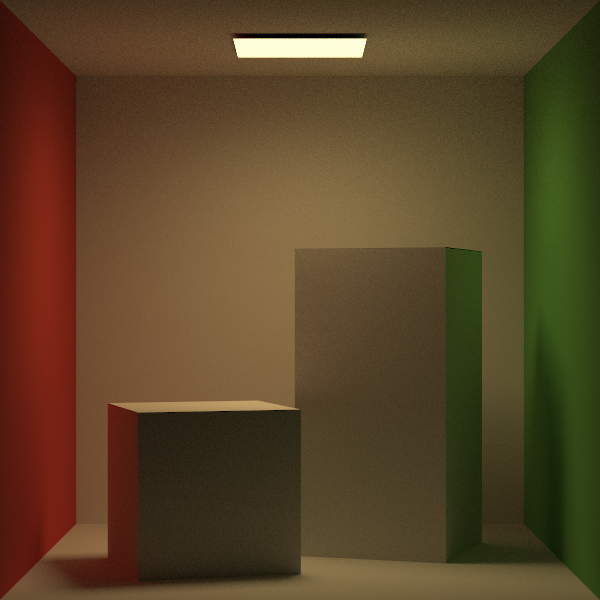
\includegraphics[width=4cm,height=4cm]{simple}
\caption{the simple result}
\end{figure}

\begin{figure}[h]
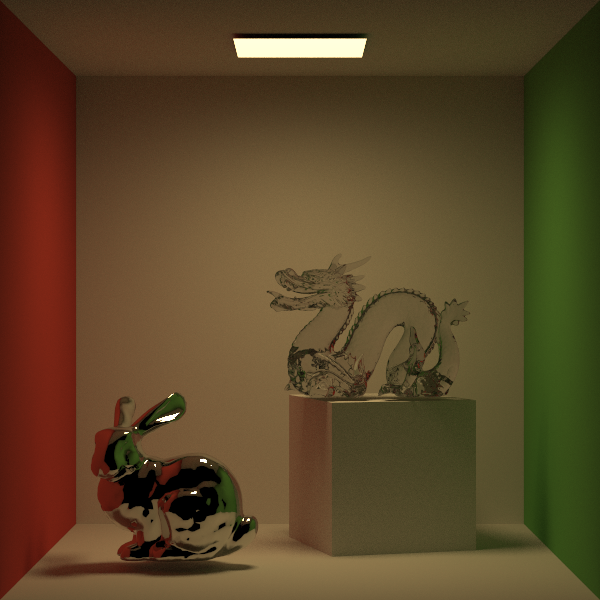
\includegraphics[width=4cm,height=4cm]{large_mesh}
\caption{the largemesh result}
\end{figure}

\end{document}